SEE APPENDIX MEI REF LATER
\subsubsection*{In Class Analysis}
\textbf{Question 1}
\begin{figure}[H]
     \centering
     \begin{subfigure}[b]{0.49\textwidth}
         \centering
         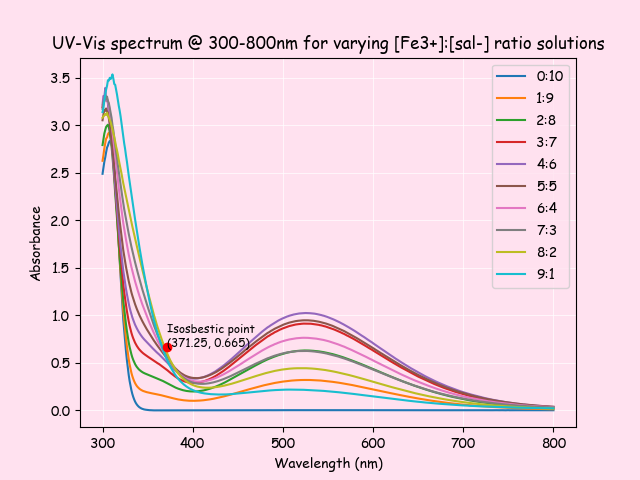
\includegraphics[width=\textwidth]{part2_q1a.png}
         \caption{RENAME}
         \label{fig:part2_q1_a}
     \end{subfigure}
     \hfill
     \begin{subfigure}[b]{0.49\textwidth}
         \centering
         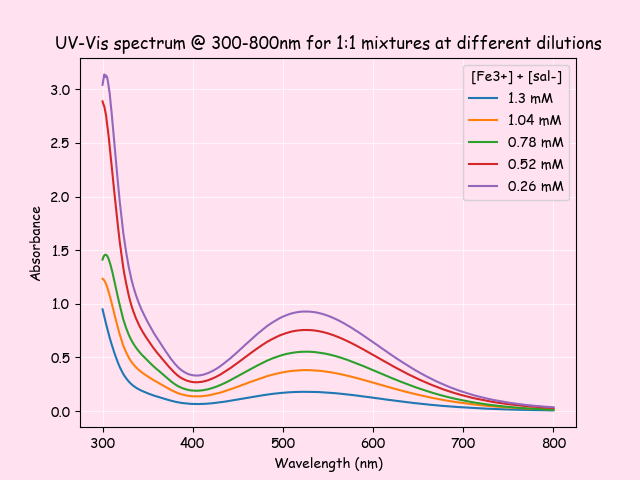
\includegraphics[width=\textwidth]{part2_q1_b.png}
         \caption{REDO}
         \label{fig:part2_q1_b}
     \end{subfigure}
     \caption{sjdfsdn}
     \label{fig:part2q1}
\end{figure}
Isosbestic point was found to be \hl{$\input{part2_q1a.txt}\unskip$}, by averaging the points of intersection for each subsequent solution for those where Fe$^{3+}$ is in excess (6:4 - 10:1). (See Appendix \ref{appx:part2_code} for Python code)
\\
\textbf{Question 2}
\begin{figure}[H]
    \centering
    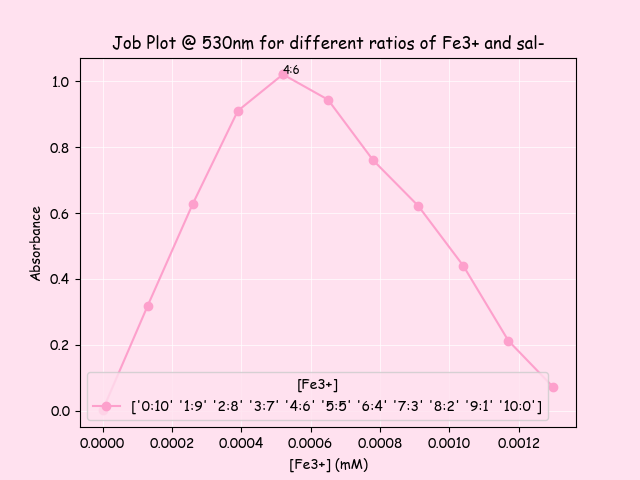
\includegraphics[width = 0.6\linewidth]{part2_q2_job_plot.png}
    \caption{Caption}
    \label{fig:part2q2}
\end{figure}
The ratio at which the peak of Job plot occured was at a ratio of \input{part2_q2.txt}\unskip. Thus, the mpirical formula of the complex was found to be:
\begin{equation}
\mathcolorbox{Lavender}{\ce{(Fe^{3+})_{4}(sal^-)_6}}
    \label{eq:emp_formula}
\end{equation}
\\
\textbf{Question 3}
\begin{figure}[H]
    \centering
    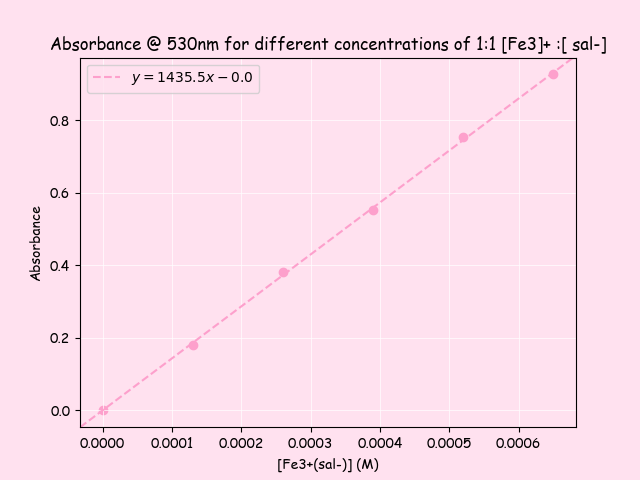
\includegraphics[width = 0.6\linewidth]{part2_q3.png}
    \caption{Caption}
    \label{fig:part2q3}
\end{figure}